\section{Results}
\paragraph{}
In this section ...

\begin{itemize}
    \item P
    \item A
\end{itemize}

\subsubsection{Paessler Webserver Stress Tool}
\paragraph{}

\textbf{ALEXANDER write here how we adjust the Paessler tool ( number of users and etc..) also include screenshot about how we customized the URLs and etc}

\subsubsection{Measuring requests \& transferred data}
\paragraph{}

\textbf{\textit{figure 3}} \& \textbf{\textit{figure 4}} below show the number of open requests as well as the number of sent and received requests in comparison with the network traffic on both the virtual and physical setups:
 
 \begin{figure}[H]
    \centering
    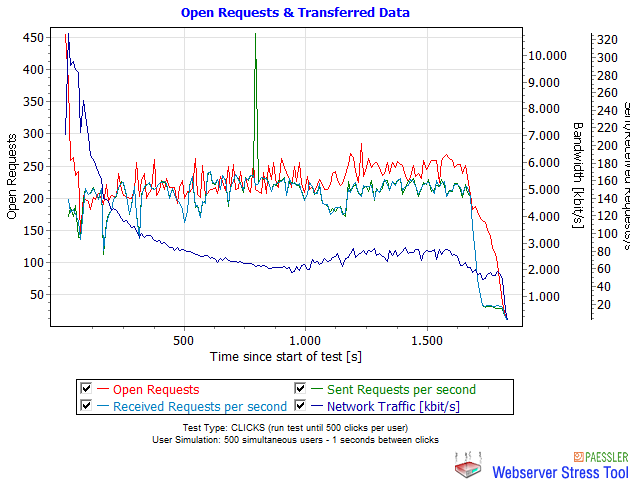
\includegraphics[width=10cm]{Pictures/graph6hw.png}
    \caption{Requests \& Transferred Data for Physical Setup}
    \label{fig:QQ3}
\end{figure}
   
 
\begin{figure}[H]
    \centering
    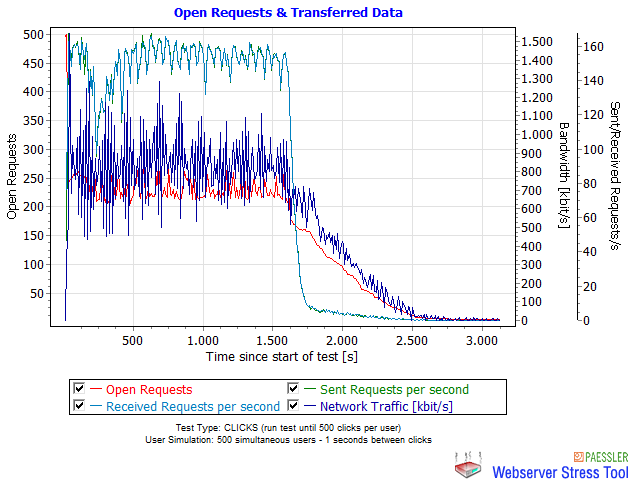
\includegraphics[width=10cm]{Pictures/graph6vm.png}
    \caption{Requests \& Transferred Data for Virtual Setup}
    \label{fig:QQ3}
\end{figure} 


\paragraph{}
\textbf{ALEXANDER also write here small conclusion about these two graphs}

\subsubsection{Measuring transferred Data \& system Memory \& CPU load}
\paragraph{}

\textbf{\textit{figure 5}} \& \textbf{\textit{figure 6}} describe the measurement for vital parameters of the machine it runs on. It can be helpful to find out if the limits of the test client have been reached testing both the virtual and physical setups:

 \begin{figure}[H]
    \centering
    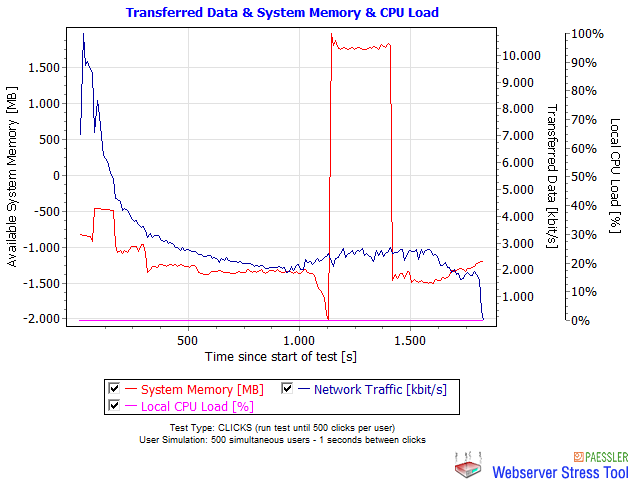
\includegraphics[width=10cm]{Pictures/ph1.png}
    \caption{Transferred Data \& System Memory \& CPU Load for Physical Setup}
    \label{fig:QQ3}
\end{figure}
   
 
\begin{figure}[H]
    \centering
    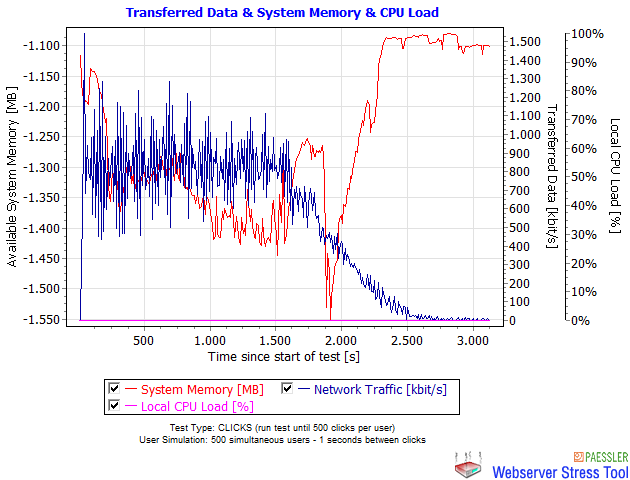
\includegraphics[width=10cm]{Pictures/vm1.png}
    \caption{Transferred Data \& System Memory \& CPU Load for Virtual Setup}
    \label{fig:QQ3}
\end{figure} 


\paragraph{}
\textbf{ALEXANDER also write here small conclusion about these two graphs}

\subsubsection{Measuring Click Time, Hits/s \& Clicks/s}
\paragraph{}

\textbf{\textit{figure 6}} \& \textbf{\textit{figure 7}} illustrate the average time a user waited for his request to be processed (including redirects, images, frames, etc., if enabled), the hits per second, and the users per clicks. 

 \begin{figure}[H]
    \centering
    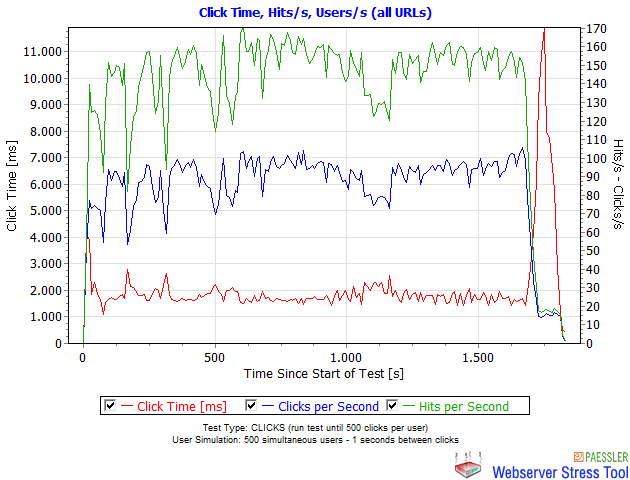
\includegraphics[width=10cm]{Pictures/ph2.png}
    \caption{Click Time, Hits/s \& Clicks/s for Physical Setup}
    \label{fig:QQ3}
\end{figure}
   
 
\begin{figure}[H]
    \centering
    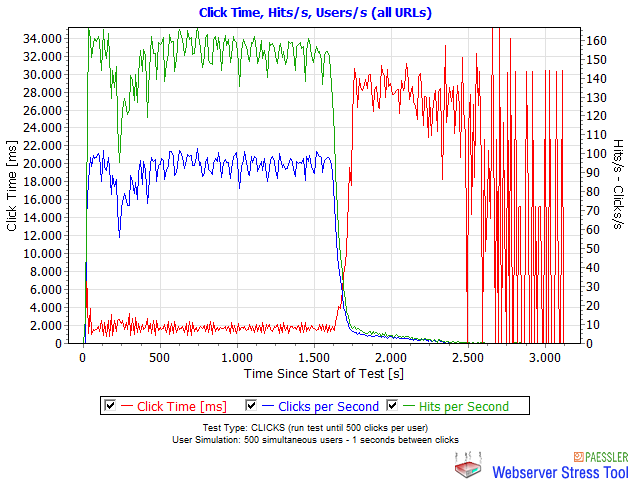
\includegraphics[width=10cm]{Pictures/vm2.png}
    \caption{Click Time, Hits/s \& Clicks/s for Virtual Setup}
    \label{fig:QQ3}
\end{figure} 


\paragraph{}
We can see that with 500 users the two lines for “clicks per second” (blue) and “hits per second” (green) differ more and more. The reason is that hits includes requests that produce errors, but clicks are only calculated from the requests that were successful.

\subsubsection{Apache Benchmark}

NOTE: Below should be an image with the test 
%%                  > WEB 1 \
%%    AB to Proxy  <         > Database 
%%                  > WEB 2 /

NOTE: Below should be an image with the test 
%%      AB to      > WEB 1 


%% Alexander : Pictures with GNU with settings %%